\documentclass[
size=17pt,
paper=smartboard,
mode=present,
display=slidesnotes,
style=paintings,
nopagebreaks,
blackslide,
fleqn]{powerdot}

% styles: sailor, paintings
% wj capsules prettybox
% mode = handout or present


\usepackage{amsmath,graphicx,color,amsfonts}
\usepackage[brazilian]{babel}
\usepackage[utf8]{inputenc}
\newcommand{\palette}{Europa}


% palettes:
%    - sailor: Sea, River, Wine, Chocolate, Cocktail 
%    - paintings: Syndics, Skater, GoldenGate, Moitessier, PearlEarring, Lamentation, HolyWood, Europa, MayThird, Charon 

\newcommand{\cursopequeno}{EC01008 AOC}
\newcommand{\cursogrande}{\Large EC01008 -- Arquitetura e organização de computadores}



\author{Ronaldo de Freitas Zampolo\\FCT-ITEC-UFPA}
\date{2023-4}


\pdsetup{
   lf = {\cursopequeno},
   rf = {Memória cache}, palette = {\palette}, randomdots={false},
   cf = {\theslide}
}


%opening
\title{\cursogrande\\ \vspace{1cm}{Memória cache}}

\begin{document}
   \maketitle[randomdots={false}]
   
   \begin{slide}{Agenda}
      \tableofcontents[content=sections]
   \end{slide}
%%%%%%%%%%%%%%%%%%%%%%%%%%%%%%%%%%%%%%%%%%%%%%%%%%%%%%
\section[slide=true]{Visão geral do sistema de memória}
\begin{slide}{Características do sistema de memória}
	\begin{itemize}
		\item Localização:
			\begin{itemize}
				\item Interna: memória principal, cache, registradores
				\item Externa: acessível por portas de E/S (discos magnético e óptico)
			\end{itemize}
		\item Capacidade: quantidade de \emph{bytes} que podem ser armazenados
		\item Unidade de transferência
			\begin{itemize}
				\item Palavra: unidade de organização da memória
				\item Unidade endereçável: palavra ou byte
				\item Unidade de transferência: número de bits lidos ou escritos
					\begin{itemize}
						\item Memória interna: palavra
						\item Memória externa: blocos
					\end{itemize}
			\end{itemize}
	\end{itemize}
\end{slide}

\begin{slide}{Características do sistema de memória}
	\begin{itemize}
		\item Método de acesso:
			\begin{itemize}
				\item Sequencial:
					\begin{itemize}
						\item Registros ordenados em sequência
						\item Para acessar um determinado registro, deve-se passar por todos entre a posição atual e a posição final
						\item Tempo de acesso variável
					\end{itemize}
				\item ``Acesso direto'':  
					\begin{itemize}
						\item Acesso direto à vizinhança + acesso sequecial à posição final
						\item Tempo de acesso variável
					\end{itemize}
				\item Acesso aleatório:
					\begin{itemize}
						\item Acesso direto à posição final
						\item Tempo de acesso constante
					\end{itemize}
			\end{itemize}
	\end{itemize}
\end{slide}

\begin{slide}{Características do sistema de memória}
	\begin{itemize}
		\item Desempenho:
			\begin{itemize}
				\item Tempo de acesso (latência):
					\begin{itemize}
						\item Tempo entre apresentação do endereço e encerramento da operação de leitura ou escrita (acesso aleatório)
						\item Tempo para posicionar o mecanismo de leitura/escrita no local desejado (acesso não-aleatório)
					\end{itemize}
				\item Tempo de ciclo de memória:
					\begin{itemize}
						\item Tempo de acesso + tempo adicional para início de novo acesso
					\end{itemize}
				\item Taxa de transferência:
					\begin{itemize}
						\item Acesso aleatório: $n/T_c$, onde $T_c$ é o tempo de ciclo
						\item Acesso não-aleatório:
							\begin{equation*}
								T_n = T_A+\frac{n}{R}
							\end{equation*}
							onde $T_n$ é o tempo médio para ler/escrever $n$ bits; $T_A$ é o tempo de acesso médio; e $R$ é a taxa de transferência (bits/segundo, bps)
					\end{itemize}
			\end{itemize}
	\end{itemize}
\end{slide}

\begin{slide}{Características do sistema de memória}
	\begin{itemize}
		\item Tipo físico:
			\begin{itemize}
				\item Memória semicondutora
				\item Memória de superfície magnética
				\item Memória óptica
				\item Memória magneto-óptica
			\end{itemize}
		\item Características físicas:
			\begin{itemize}
				\item Memória volátil: o conteúdo é perdido com quando a energia é retirada
				\item Memória não-volátil: o conteúdo é preservado mesmo sem alimentação elétrica
				\item Memória não-apagável: conteúdo não pode ser alterado
			\end{itemize}
	\end{itemize}
\end{slide}

\begin{slide}{Hierarquia de memória}
	As três perguntas críticas (há um compromisso aqui):
	\begin{itemize}
		\item Qual a capacidade (quanto bits podem ser armazenados)?
		\item Quão rápido o ciclo de memória?
		\item Qual o custo por bit?
	\end{itemize}\pause
	\twocolumn{
		\begin{itemize}
			\item De cima para baixo na hierarquia:
				\begin{itemize}
					\item Diminuição do custo por bit
					\item Aumento da capacidade
					\item Aumento do tempo de acesso
					\item \textbf{Diminuição da frequência de acesso}: princípio da localidade de referência \pause
						\begin{itemize}
							\item Referências à memória tendem a restringir-se a um cluster
							\item Longo prazo: cluster muda
							\item Curto prazo: cluster fixo
						\end{itemize}
				\end{itemize}
		\end{itemize}
	}
	{
		\centering
		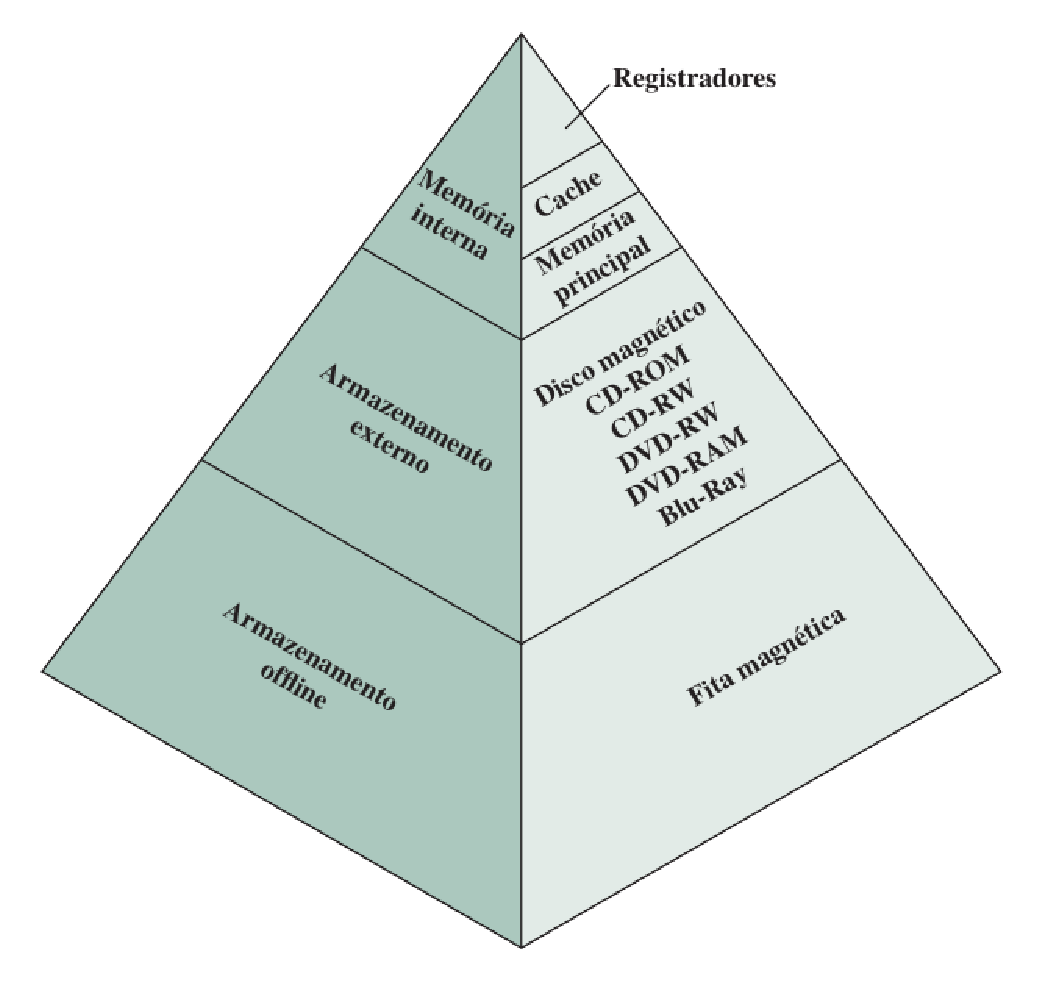
\includegraphics[width=0.95\textwidth]{figs/piramide2}
	}
\end{slide}

\begin{slide}{Sistema com dois níveis de memória}
 Considere que:
 %\footnotesize
    \begin{itemize}
       \item O sistema de memória de uma máquina possui apenas dois níveis: 1 e 2;
       \item Os níveis 1 e 2 possuem tempos de acesso $T_1$ e $T_2$, respectivamente;
       \item Se uma determinada palavra que precisa ser acessada encontra-se no nível 1, o processador a acessa diretamente ($T_1$);
       \item Se a palavra estiver no nível 2, ela é primeiro transferida para o nível 1 e depois acessada pelo processador ($T_1+T_2$);
       \item Determine o tempo médio de acesso, se a razão de acerto do nível 1 for de: a) 0,1; b) 0,5; c) 0,9;\pause
       \item Determine uma equação e trace o gráfico correspondente do tempo médio de acesso em função da razão de acerto do nível 1 .\pause
       \item Generalize a equação para o caso de uma memória de $n$ níveis.
    \end{itemize}
 \end{slide}
\begin{slide}{Sistema com dois níveis de memória}
	Gráfico do tempo médio de acesso para memória de dois níveis em função da razão de acerto\\
	\centering
	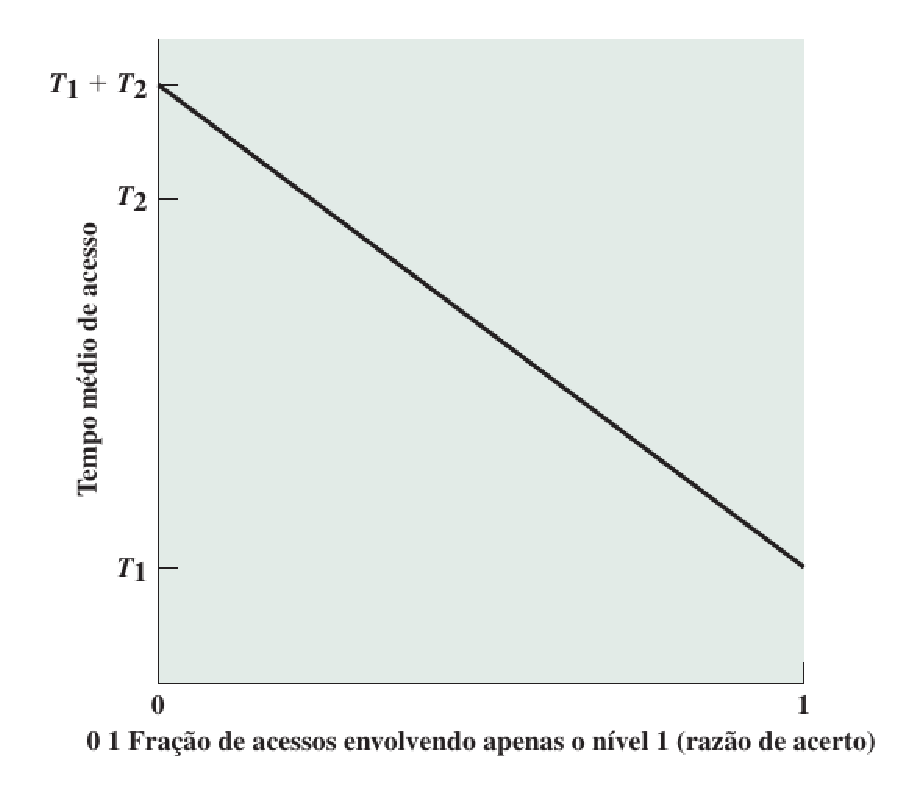
\includegraphics[width=0.55\textwidth]{figs/dois-niveis-grafico}
 \end{slide}

\begin{slide}{Visibilidade}
\begin{itemize}
   \item A cache é normalmente invisível para o programador ou processador;
   \item Serve para organizar a movimentação de dados entre memória principal e os registradores do processador;
   \item Objetivo: melhorar o desempenho do sistema
\end{itemize}
\end{slide}

\section[slide=true]{Princípios da memória cache}
\begin{slide}{Princípios da memória cache}
\begin{itemize}
   \item A cache contém uma cópia de parte da memória principal;
   \item Quando o processador precisa acessar uma palavra da memória:
   \begin{itemize}
      \item É feita uma verificação se a palavra está na cache. Se estiver, a palavra é acessada.
      \item Se não estiver, um \emph{bloco de palavras} é transferido da memória principal para a cache e depois a palavra é fornecida ao processador.
   \end{itemize}
   \item Em razão do \emph{princípio da localidade de referência}, haverá futuras referências ao mesmo endereço ou aos seus vizinhos (membros do mesmo bloco).
\end{itemize}
\end{slide}

\begin{slide}{Cache e memória principal}
	\begin{itemize}
		\item Cache única\\
			{\centering
			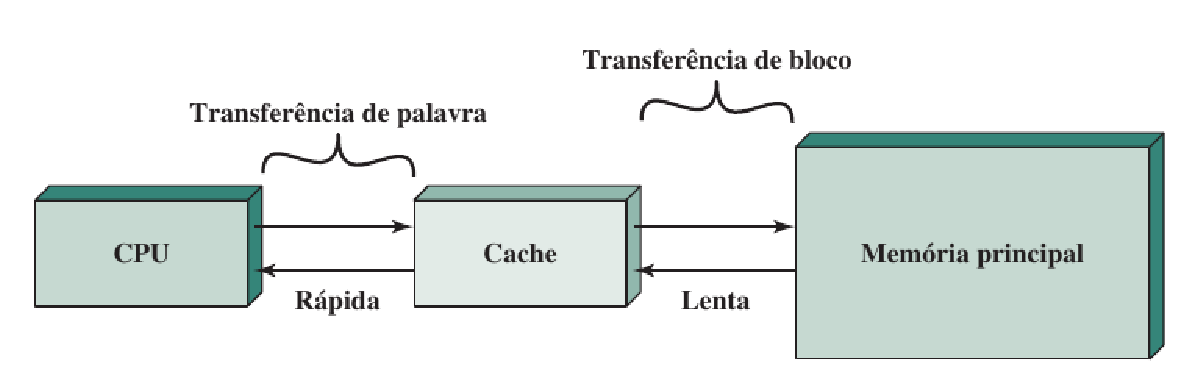
\includegraphics[width=0.65\textwidth]{figs/cache-unica}}
		\item Cache com três níveis\\
			{\centering
			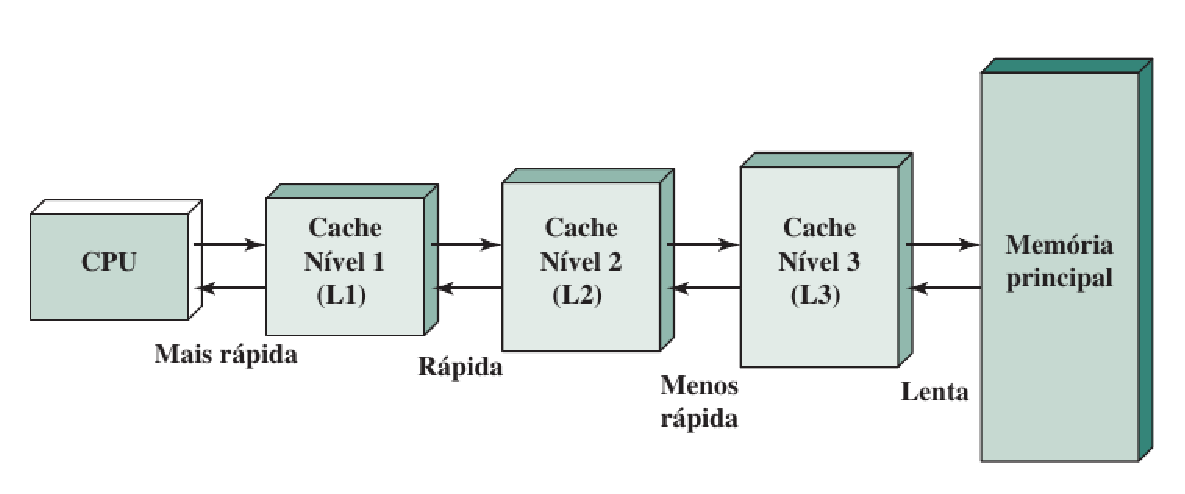
\includegraphics[width=0.65\textwidth]{figs/cache-tres-niveis}}
	\end{itemize}
\end{slide}

\begin{slide}{Estrutura de organização da cache/memória}
	\twocolumn{
	\small
	\begin{itemize}
		\item Memória principal:
			\begin{itemize}
				\item Número total de endereços: $2^n$
				\item Cada endereço armazena uma palavra
				\item Para fins de transferência com a memória cache, pode ser vista como um conjunto de blocos de $K$ palavras
				\item Número total de blocos: $M = 2^n/K$
			\end{itemize}
		\item Memória cache:
			\begin{itemize}
				\item É organizada em linhas
				\item Cada linha armazena:
					\begin{itemize}
						\item Um bloco ($K$ palavras) da memória principal
						\item Uma TAG: permite verificar o endereço original (o da memória principal) do bloco armazenado
						\item Bits de controle: indicam se a linha foi alterada
					\end{itemize}\pause
				\item Como $C<<M$, haverá concorrência entre blocos de memória por linhas da cache
			\end{itemize}
	\end{itemize}
	}
	{
   			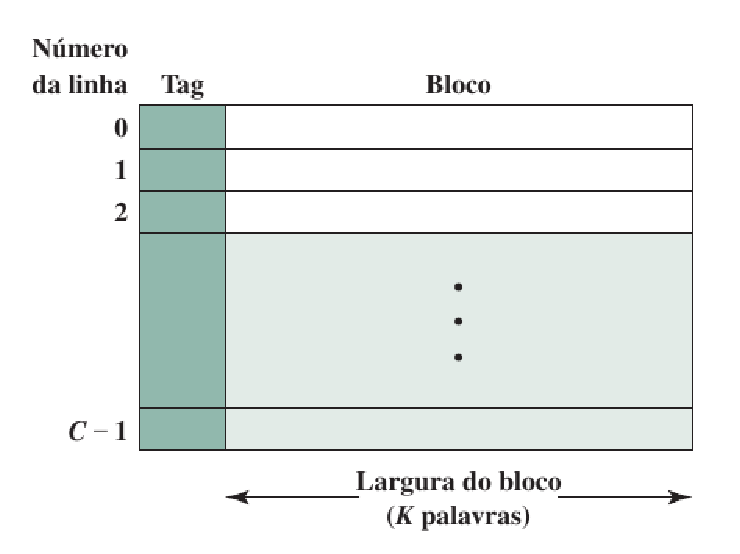
\includegraphics[width=0.45\textwidth]{figs/estrutura-cache}
			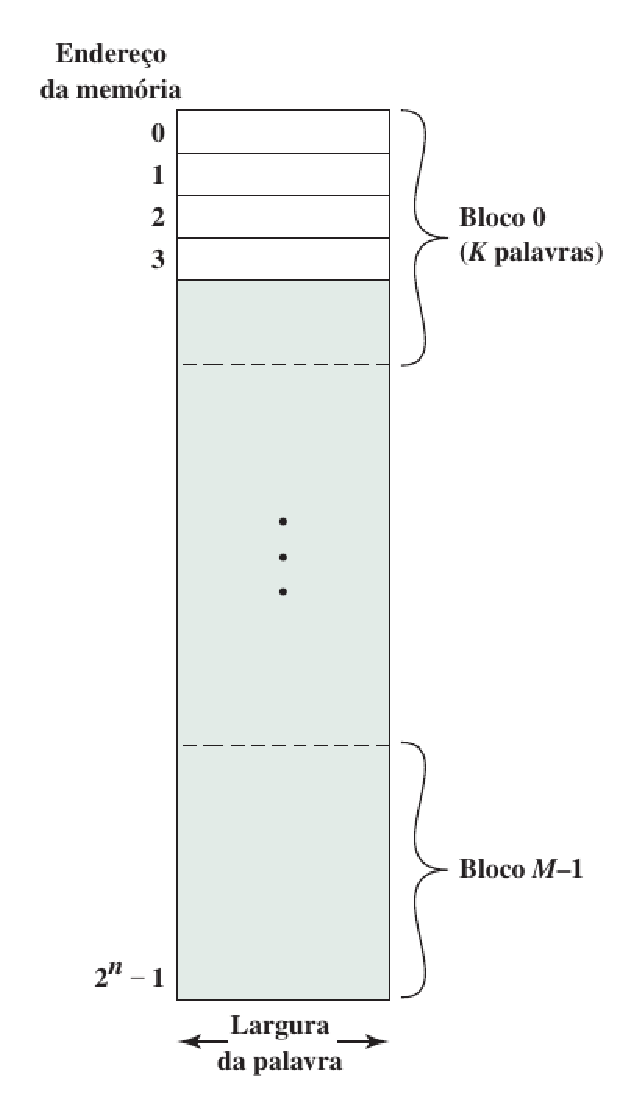
\includegraphics[width=0.50\textwidth]{figs/estrutura-memoria-principal}
	}
\end{slide}

\begin{slide}{Operação de leitura}
	Etapas para leitura de uma palavra em memória
	\begin{center}
		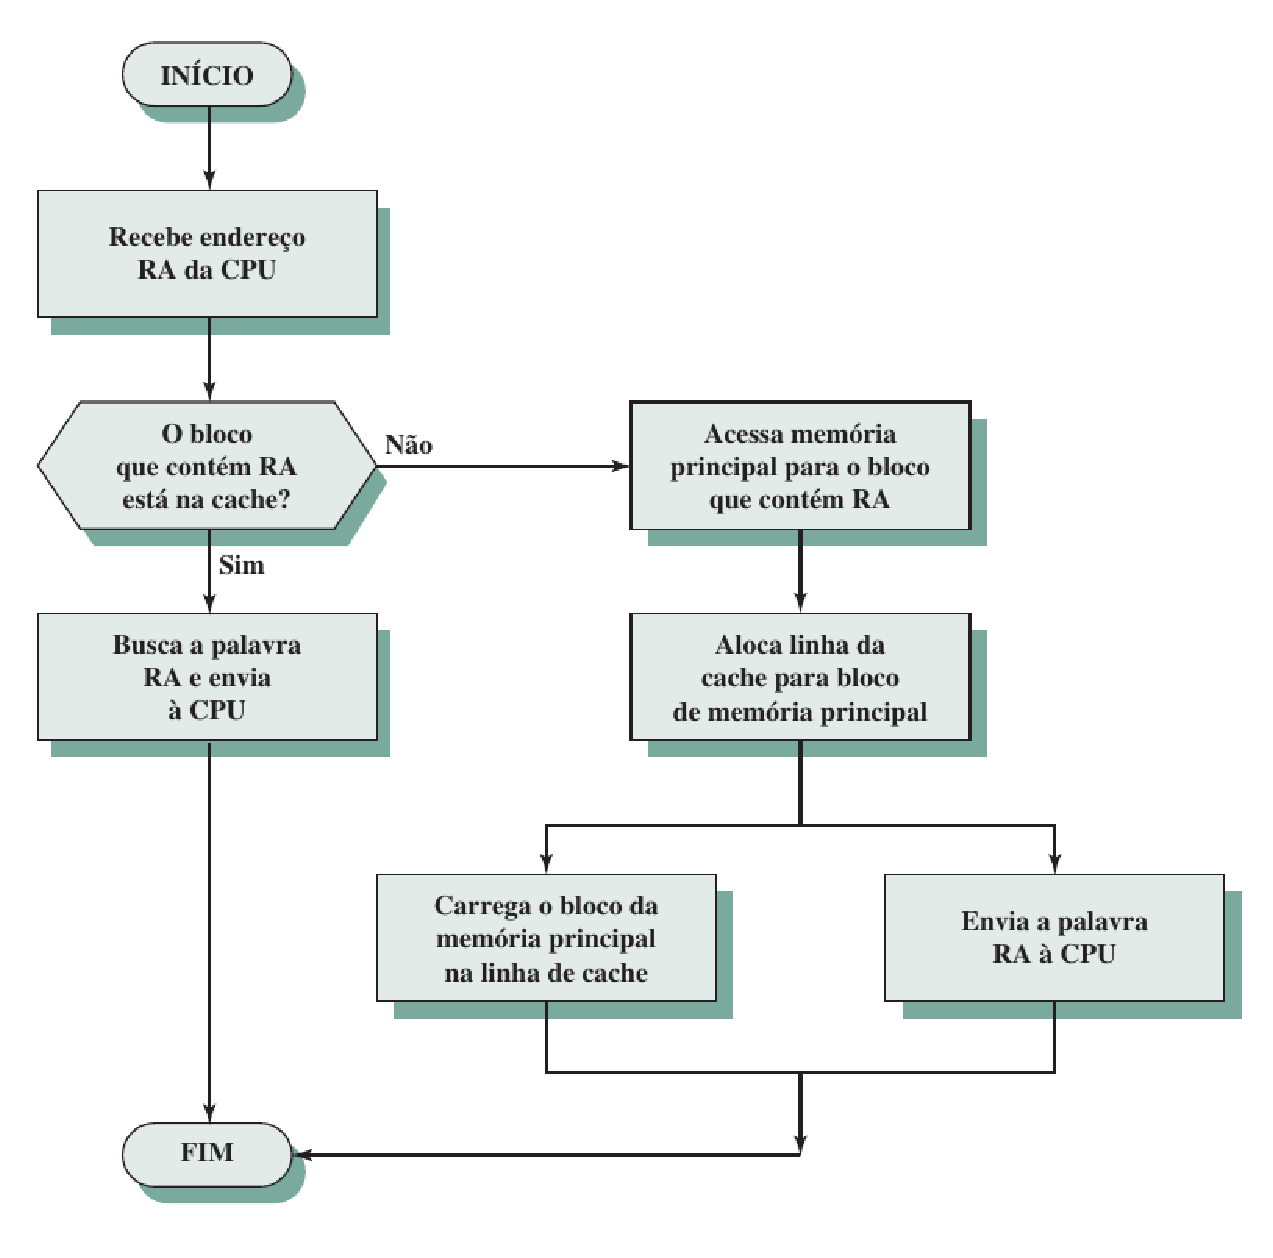
\includegraphics[width=0.50\textwidth]{figs/leitura-cache}
	\end{center}
\end{slide}

\begin{slide}{Organização}
	Organização típica de uma memória cache
	\begin{center}
		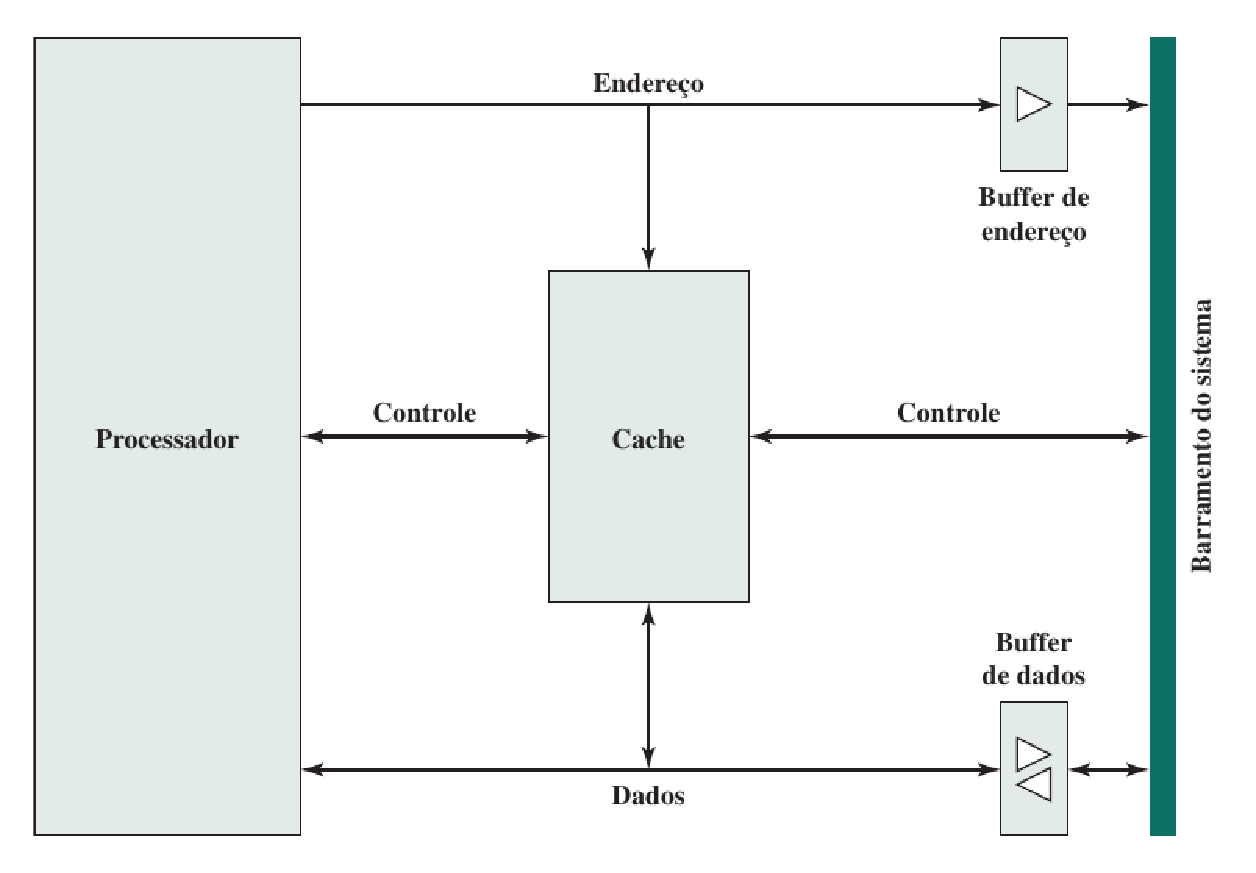
\includegraphics[width=0.70\textwidth]{figs/organizacao-tipica-cache}
	\end{center}
\end{slide}

\section[slide=true]{Elementos de projeto da memória cache}
\begin{slide}{Principais elementos em um projeto de memória cache}
	\twocolumn{
	\begin{itemize}
		\item Endereço de cache
			\begin{itemize}
				\item Cache lógica
				\item Cache física
			\end{itemize}
		\item Tamanho de cache
		\item Função/estratégia de mapeamento
			\begin{itemize}
				\item Mapeamento direto
				\item Mapeamento associativo
				\item Mapeamento associativo em conjunto
			\end{itemize}
		\item Tamanho da linha
	\end{itemize}
	}
	{
	\begin{itemize}
		\item Algoritmo de substituição
			\begin{itemize}
				\item O menos recentemente usado (LRU)
				\item Primeiro a entrar primeiro a sair (FIFO)
				\item O menos frequentemente usado (LFU)
				\item Aleatório
			\end{itemize}
		\item Política de escrita
			\begin{itemize}
				\item \emph{Write through}
				\item \emph{Write back}
			\end{itemize} 
		\item Número de caches
			\begin{itemize}
				\item Única ou de dois níveis
				\item Unificada ou separada
			\end{itemize}
	\end{itemize}
	}
\end{slide}

\begin{slide}{Endereços de cache}
\begin{itemize}
	\item Memória virtual: acesso à memória por endereços lógicos (não físicos)
	\item Cache lógica: mais rápido; deve ser esvaziada a cada mudança de contexto
		\begin{center}
			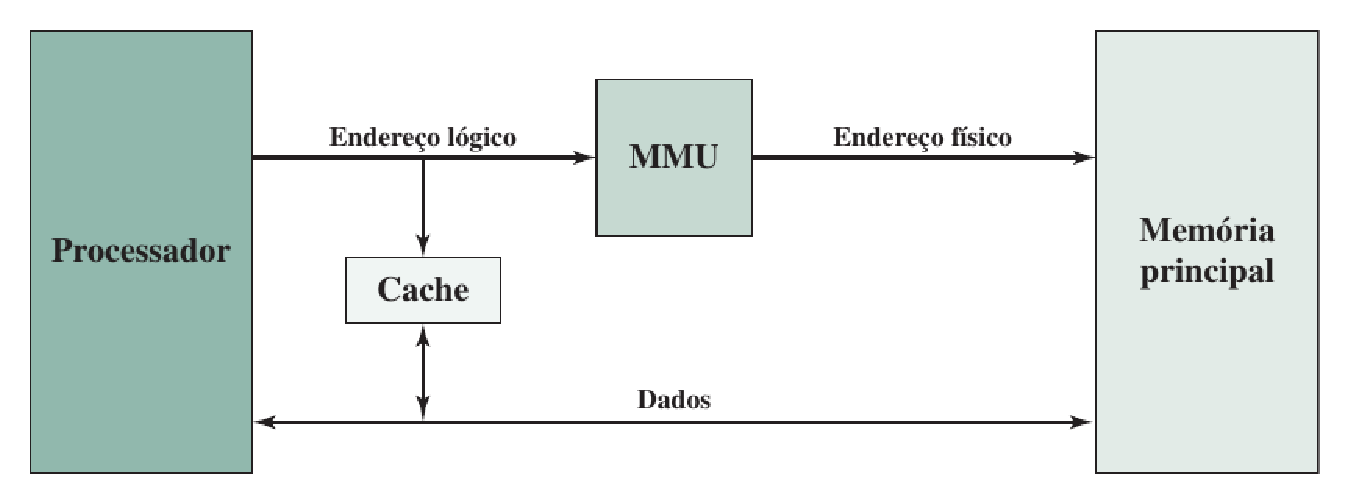
\includegraphics[width=0.5\textwidth]{figs/cache-logica}
		\end{center}
	\item Cache física: mais lento; cache continua válida quando há mudança de contexto
		\begin{center}
			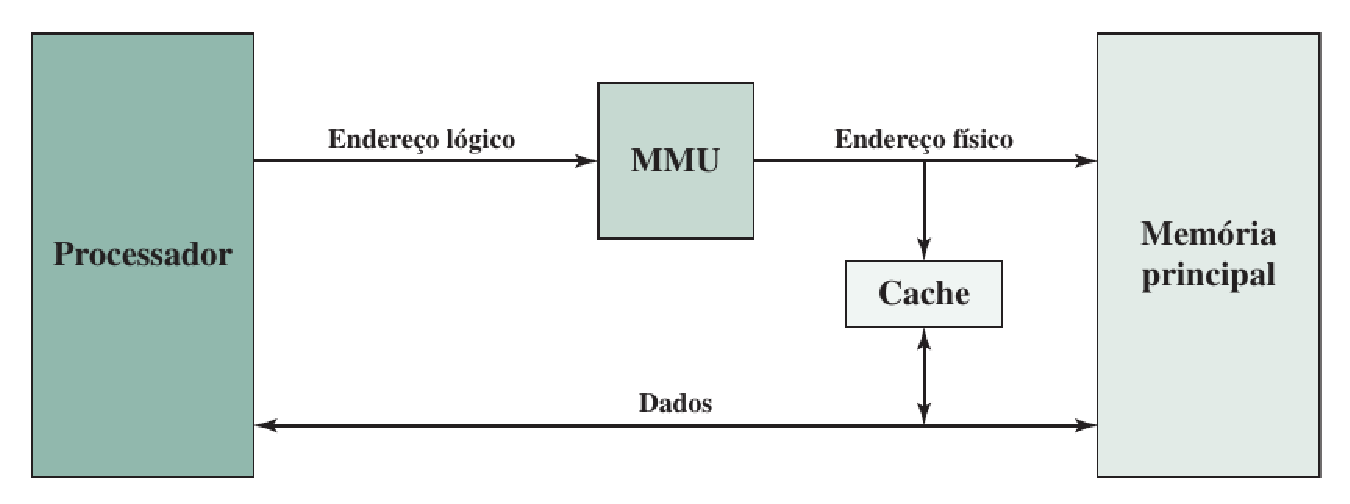
\includegraphics[width=0.5\textwidth]{figs/cache-fisica}
		\end{center}
\end{itemize}
\end{slide}

\begin{slide}{Tamanho da cache}
Deseja-se que o tamanho da cache seja:
\begin{itemize}
 \item Pequeno o suficiente para que o custo médio por bit seja próximo do custo da memória principal isolada;
 \item Grande o suficiente para que o tempo de acesso médio seja próximo do tempo de acesso da memória cache isolada.
\end{itemize}
\end{slide}

\begin{slide}{Função de mapeamento}
\begin{itemize}
%\scriptsize
 \item Mapeamento direto:
 \begin{itemize}
    \item Técnica mais simples
    \item Cada bloco da memória principal é possível de mapeado para apenas uma linha específica da cache;
    \item Problema se blocos frequentes forem concorrentes pela mesma linha da cache (ver \emph{selective victim cache})
    \item linha da cache:  $i \leftarrow j\mod m$
 \end{itemize}\pause
 \item Mapeamento associativo:
 \begin{itemize}
    \item Cada bloco da memória principal pode ser mapeado para qualquer linha da cache;
    \item Flexível, mas acarreta complexidade aos circuitos de busca de palavras na cache;
 \end{itemize}\pause
 \item Mapeamento associativo em conjunto:
 \begin{itemize}
    \item Meio termo entre as duas estratégias anteriores.
 \end{itemize}
\end{itemize}
\end{slide}

\begin{slide}{Mapeamento direto}
	Mapeamento entre memória principal e memória cache
	\begin{center}
		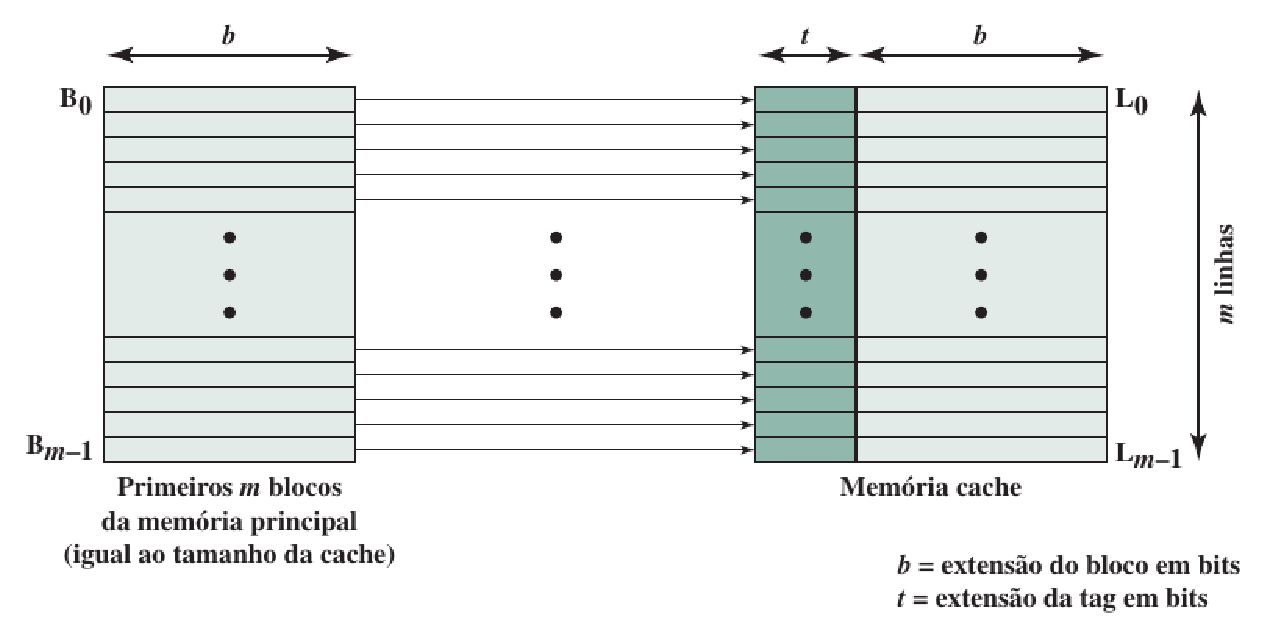
\includegraphics[width=0.75\textwidth]{figs/mapeamento-direto}
	\end{center}
\end{slide}

\begin{slide}{Mapeamento direto}
	Exemplo de mapeamento direto
	\begin{center}
		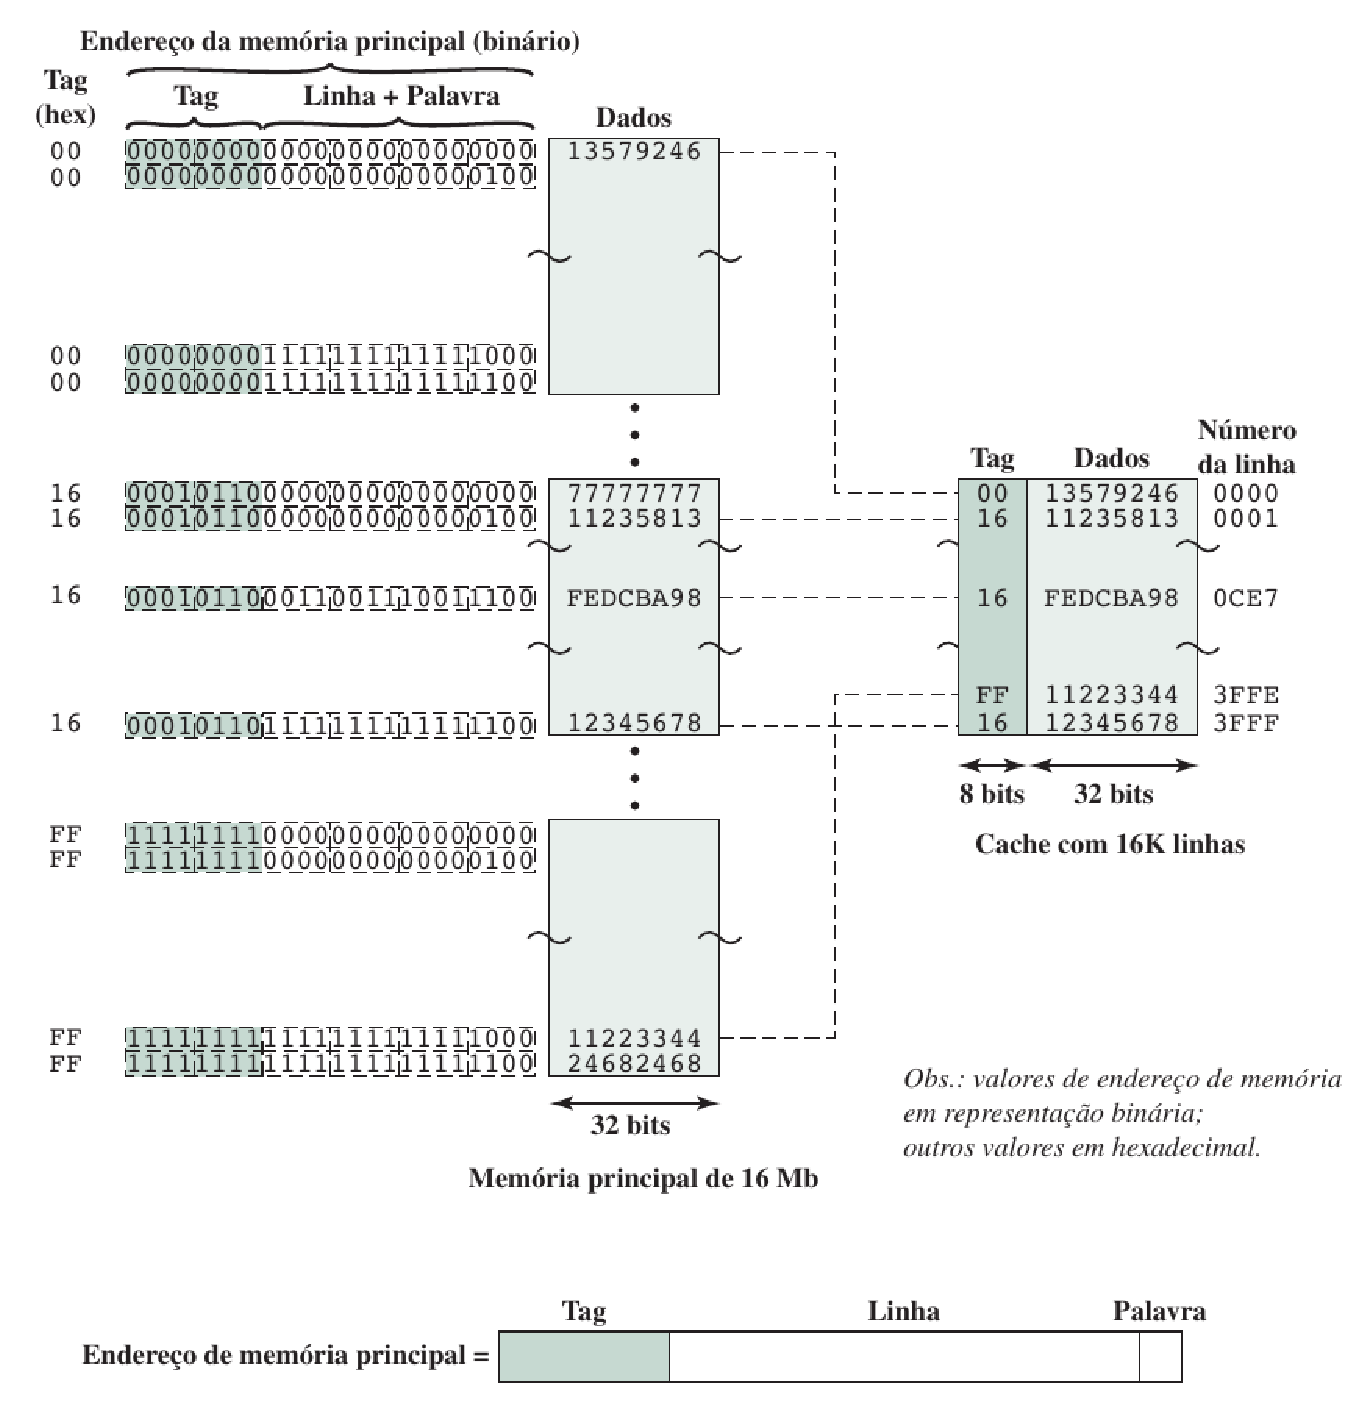
\includegraphics[height=0.5\textwidth]{figs/exemplo-direto}
	\end{center}
\end{slide}

\begin{slide}{Mapeamento direto}
	Organização de uma cache com  mapeamento direto
	\begin{center}
		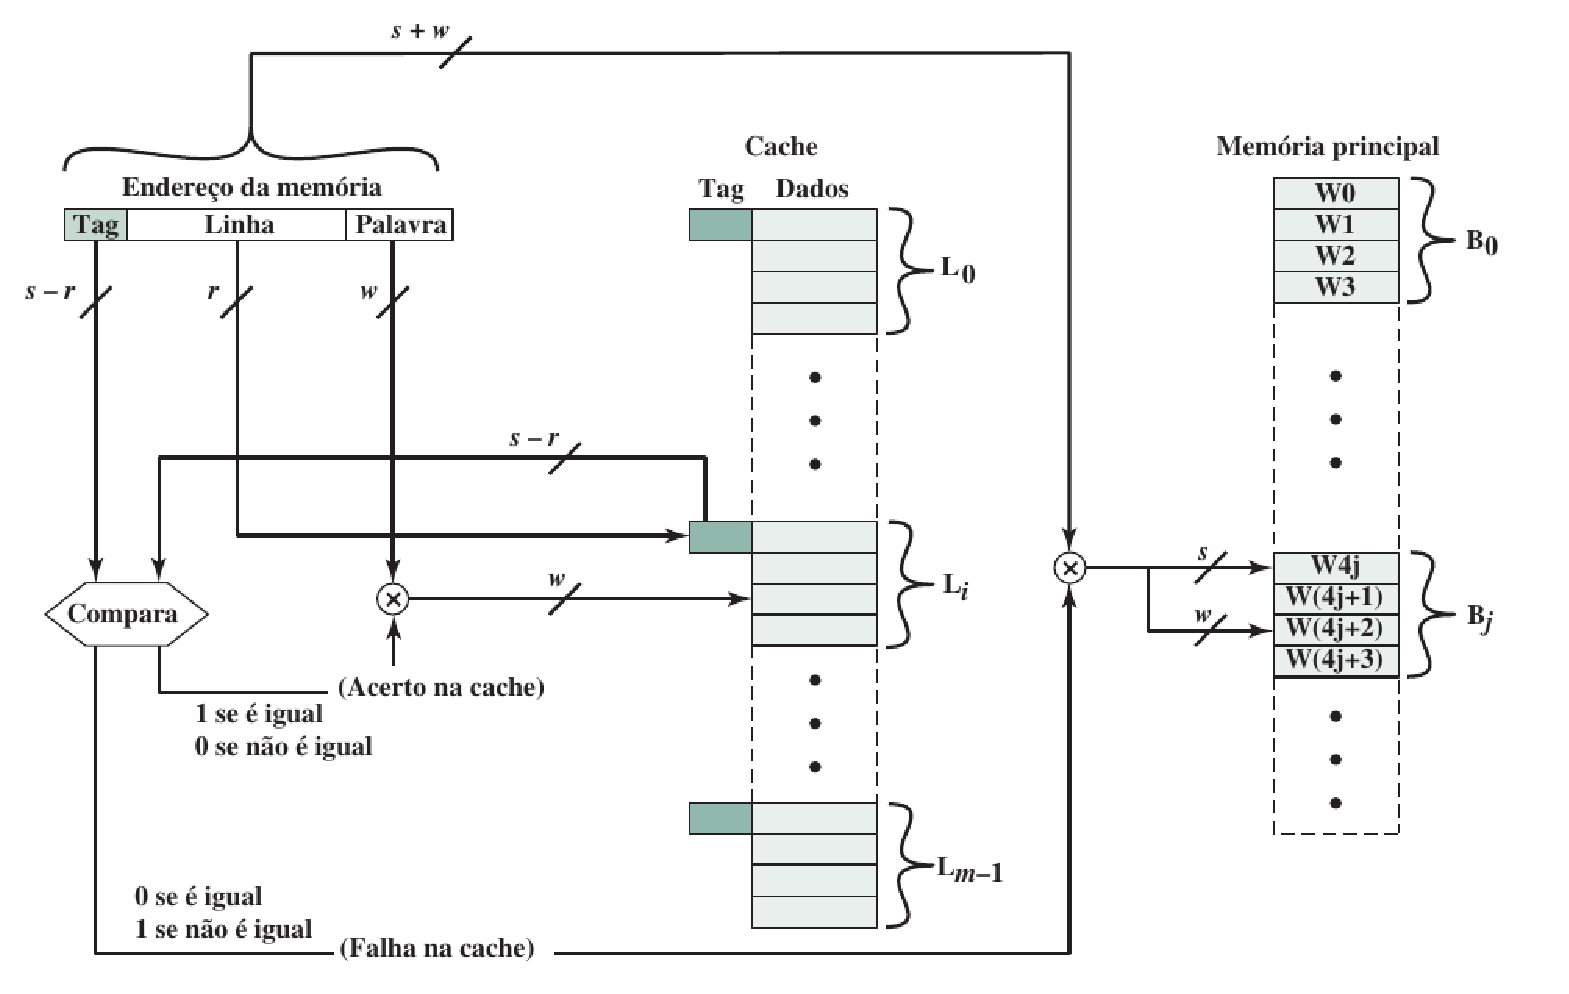
\includegraphics[height=0.5\textwidth]{figs/organizacao-direto}
	\end{center}
\end{slide}

\begin{slide}{Mapeamento associativo}
	Mapeamento entre memória principal e memória cache
	\begin{center}
		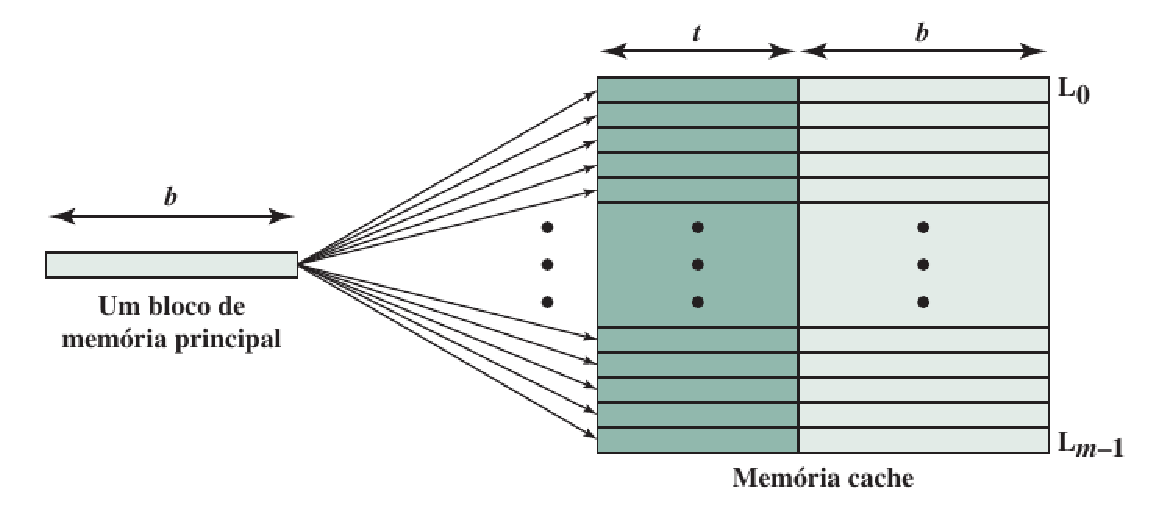
\includegraphics[width=0.75\textwidth]{figs/mapeamento-associativo}
	\end{center}
\end{slide}

\begin{slide}{Mapeamento associativo}
	Exemplo de mapeamento associativo
	\begin{center}
		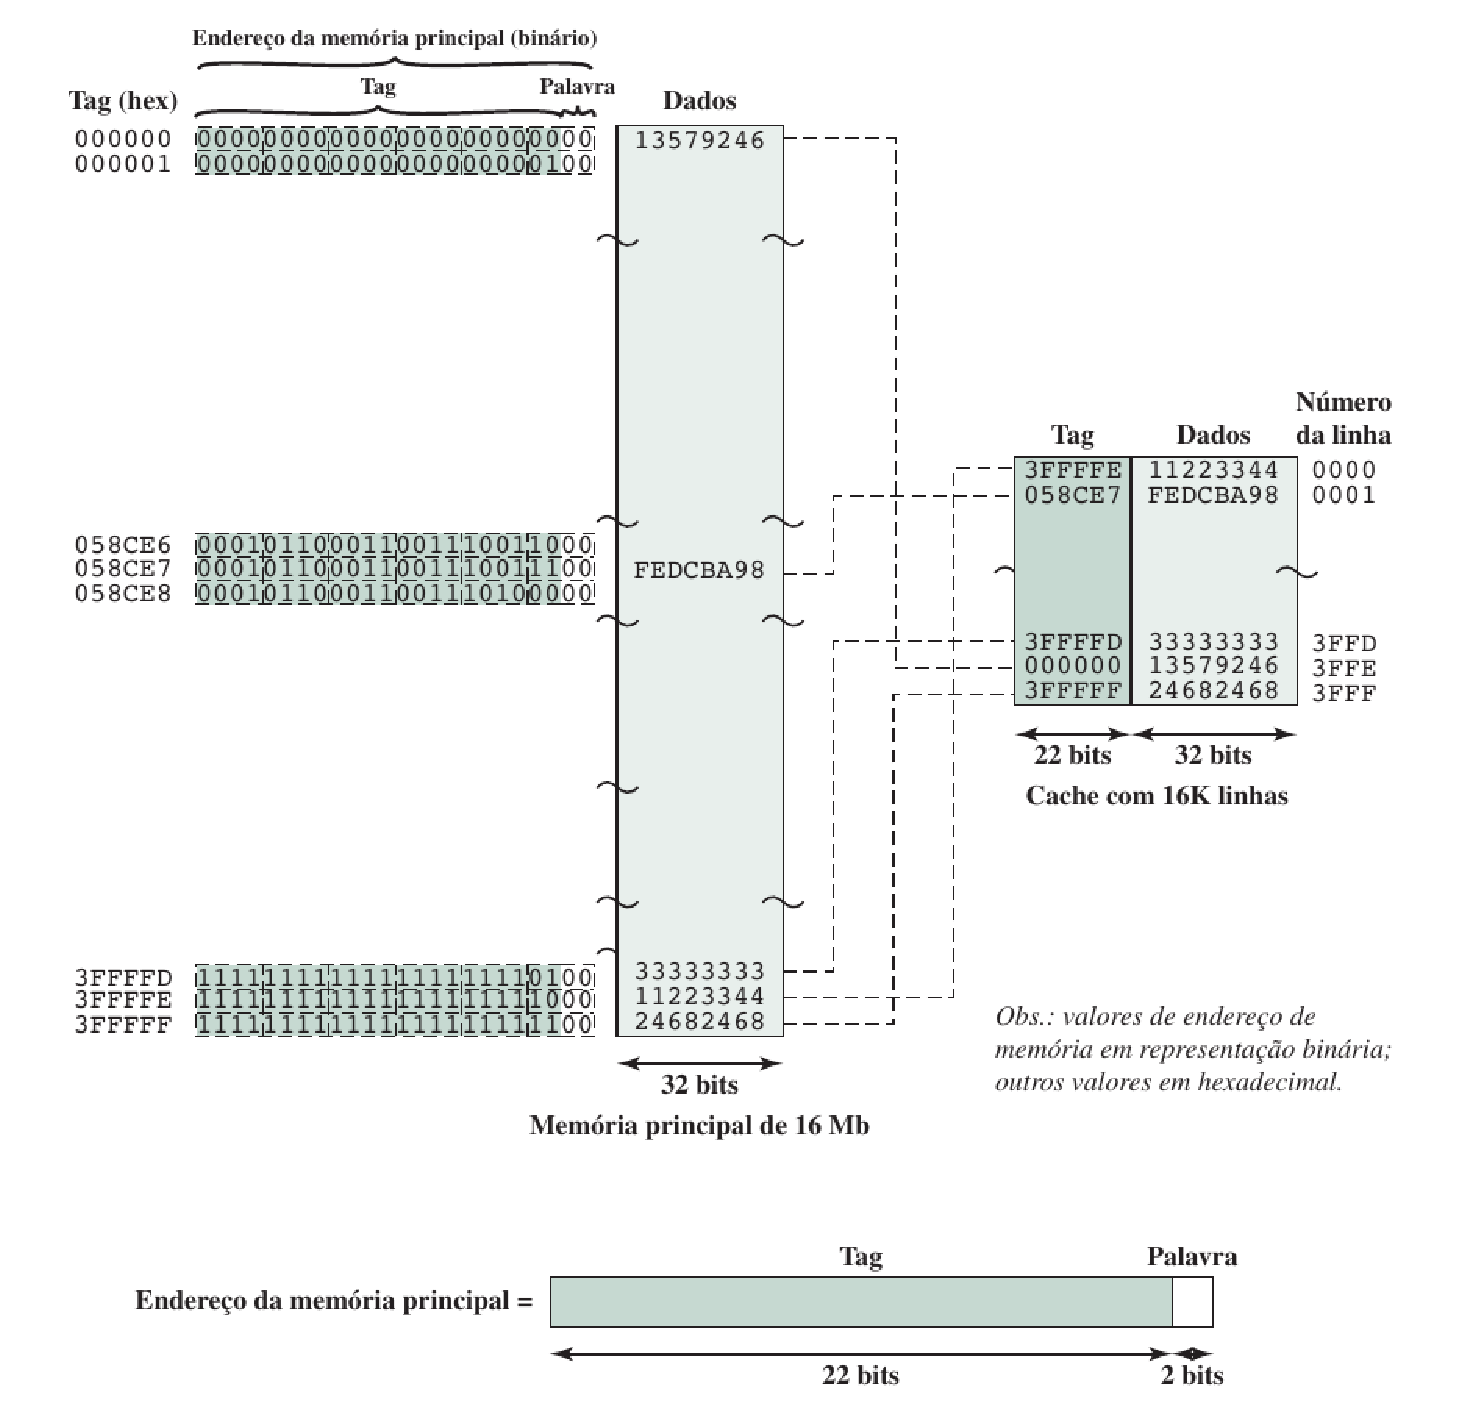
\includegraphics[height=0.5\textwidth]{figs/exemplo-associativo}
	\end{center}
\end{slide}

\begin{slide}{Mapeamento associativo}
	Organização de uma cache com mapeamento associativo
	\begin{center}
		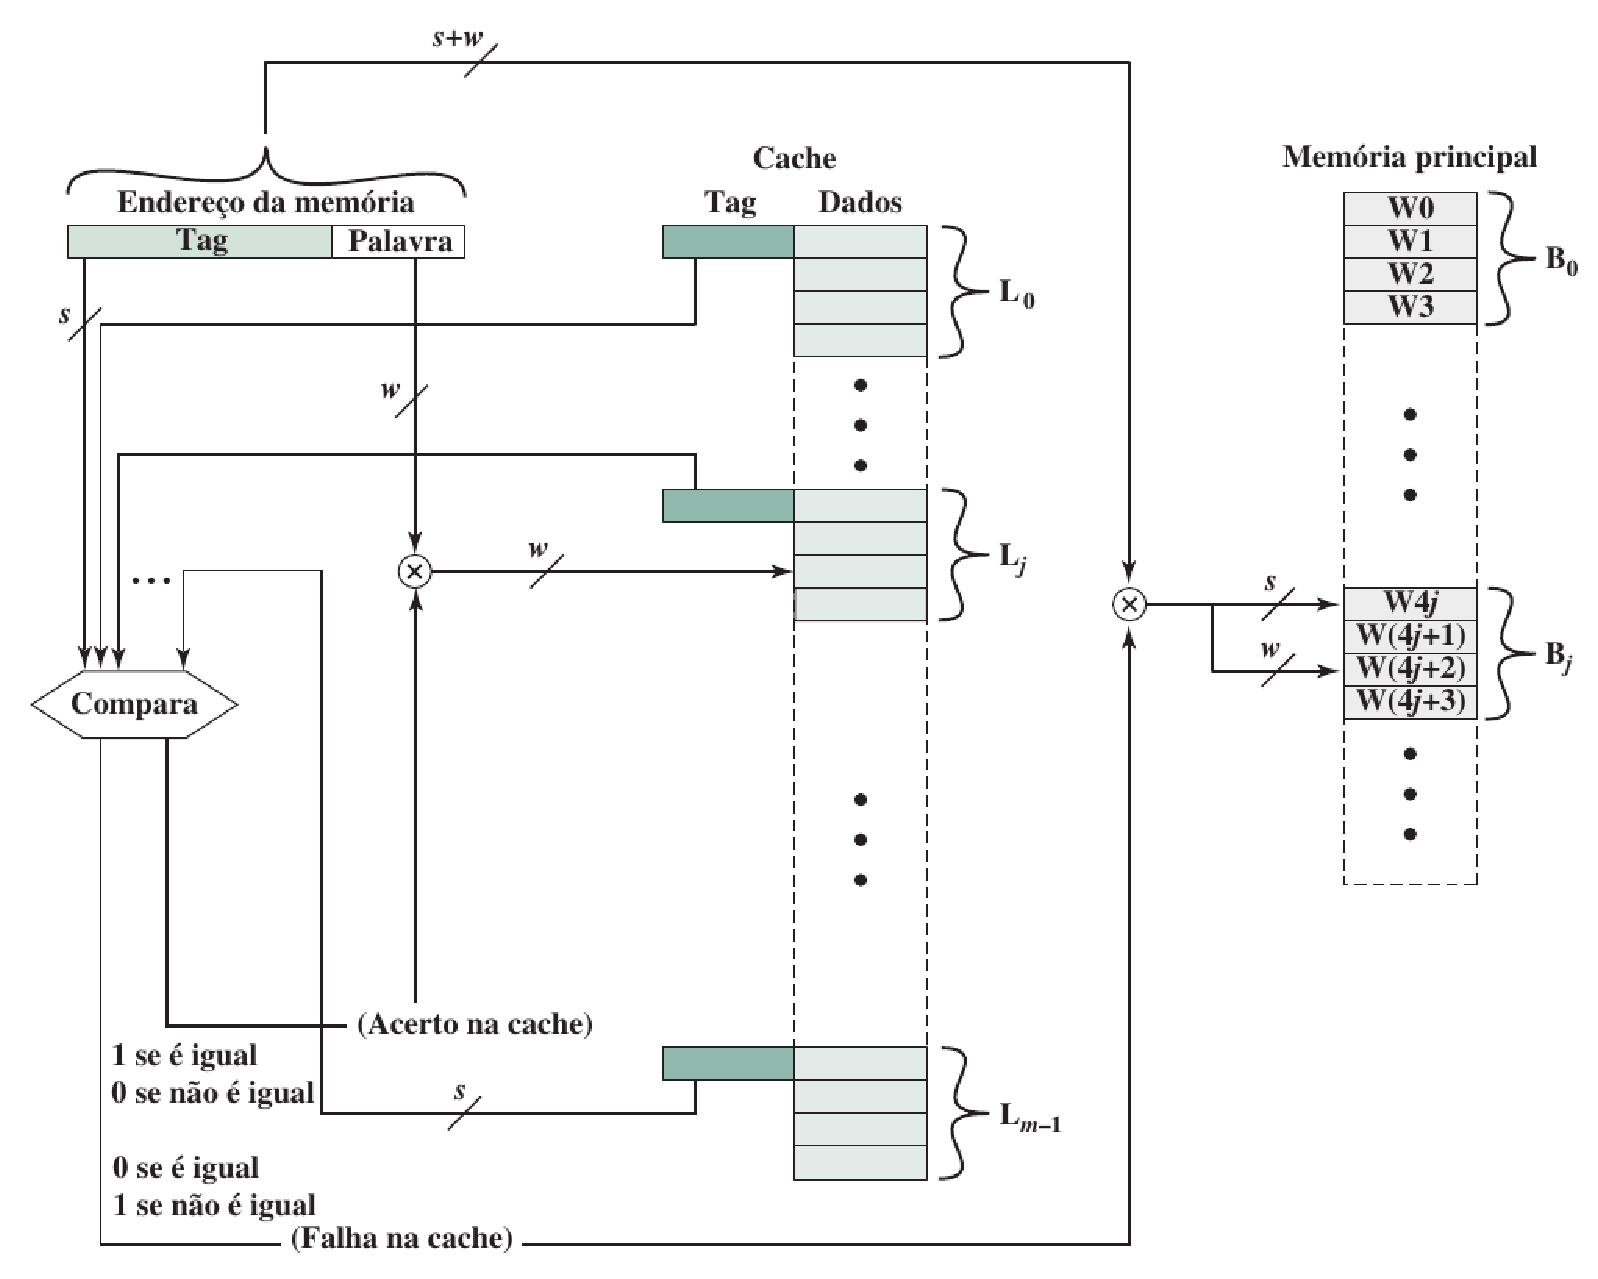
\includegraphics[height=0.5\textwidth]{figs/organizacao-associativo}
	\end{center}
\end{slide}

\begin{slide}{Mapeamento associativo em conjunto}
	Mapeamento entre memória principal e memória cache -- visão 1
	\begin{center}
		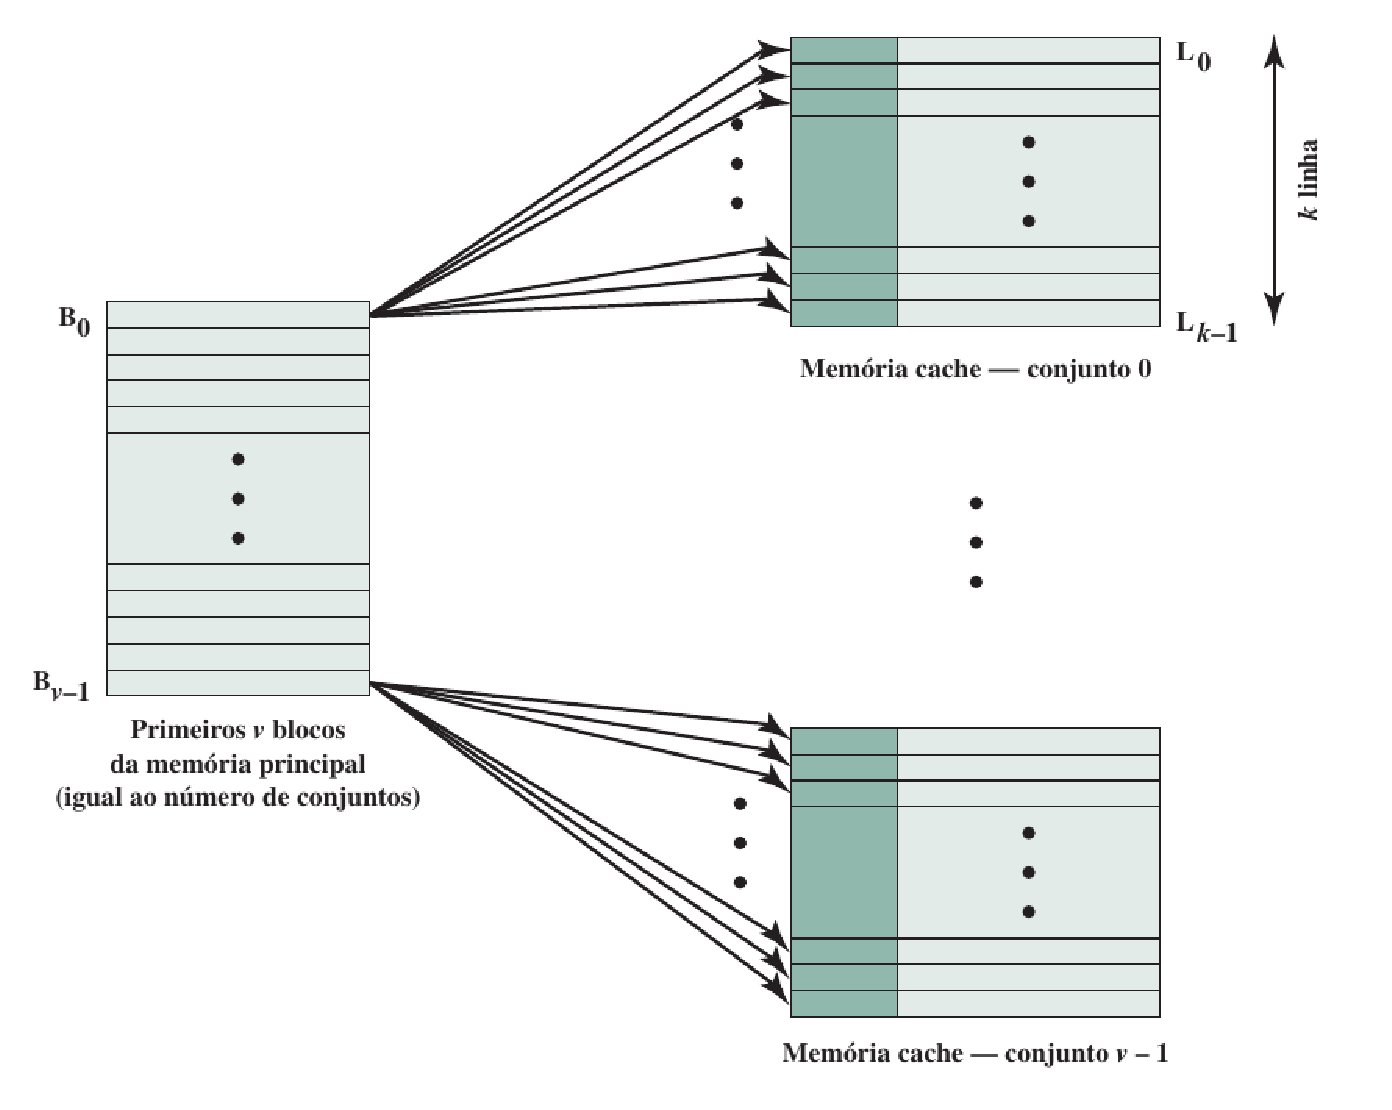
\includegraphics[width=0.55\textwidth]{figs/associativo-conj-01}
	\end{center}
\end{slide}

\begin{slide}{Mapeamento associativo em conjunto}
	Mapeamento entre memória principal e memória cache -- visão 2
	\begin{center}
		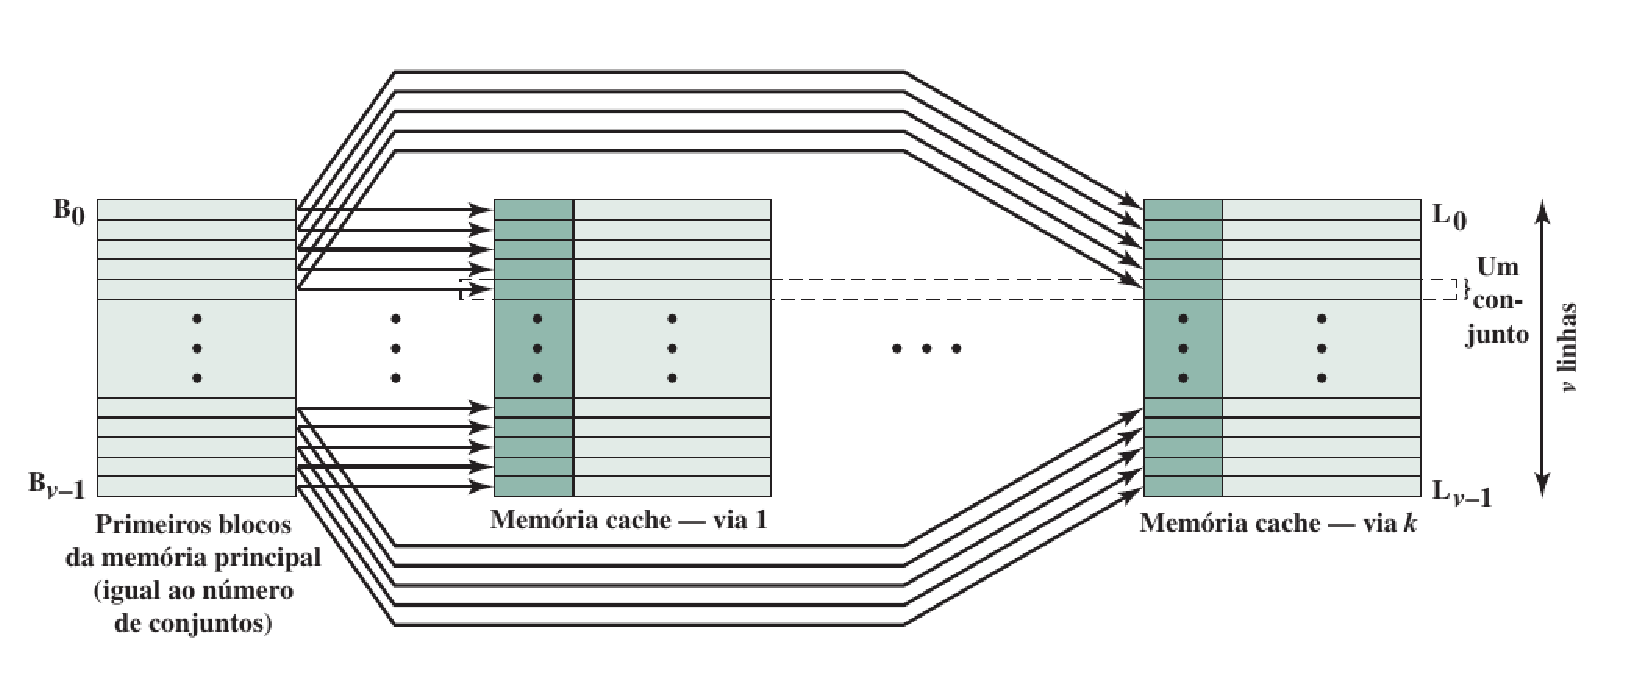
\includegraphics[width=0.75\textwidth]{figs/associativo-conj-02}
	\end{center}
\end{slide}

\begin{slide}{Mapeamento associativo em conjunto}
	Exemplo de mapeamento associativo em conjunto
	\begin{center}
		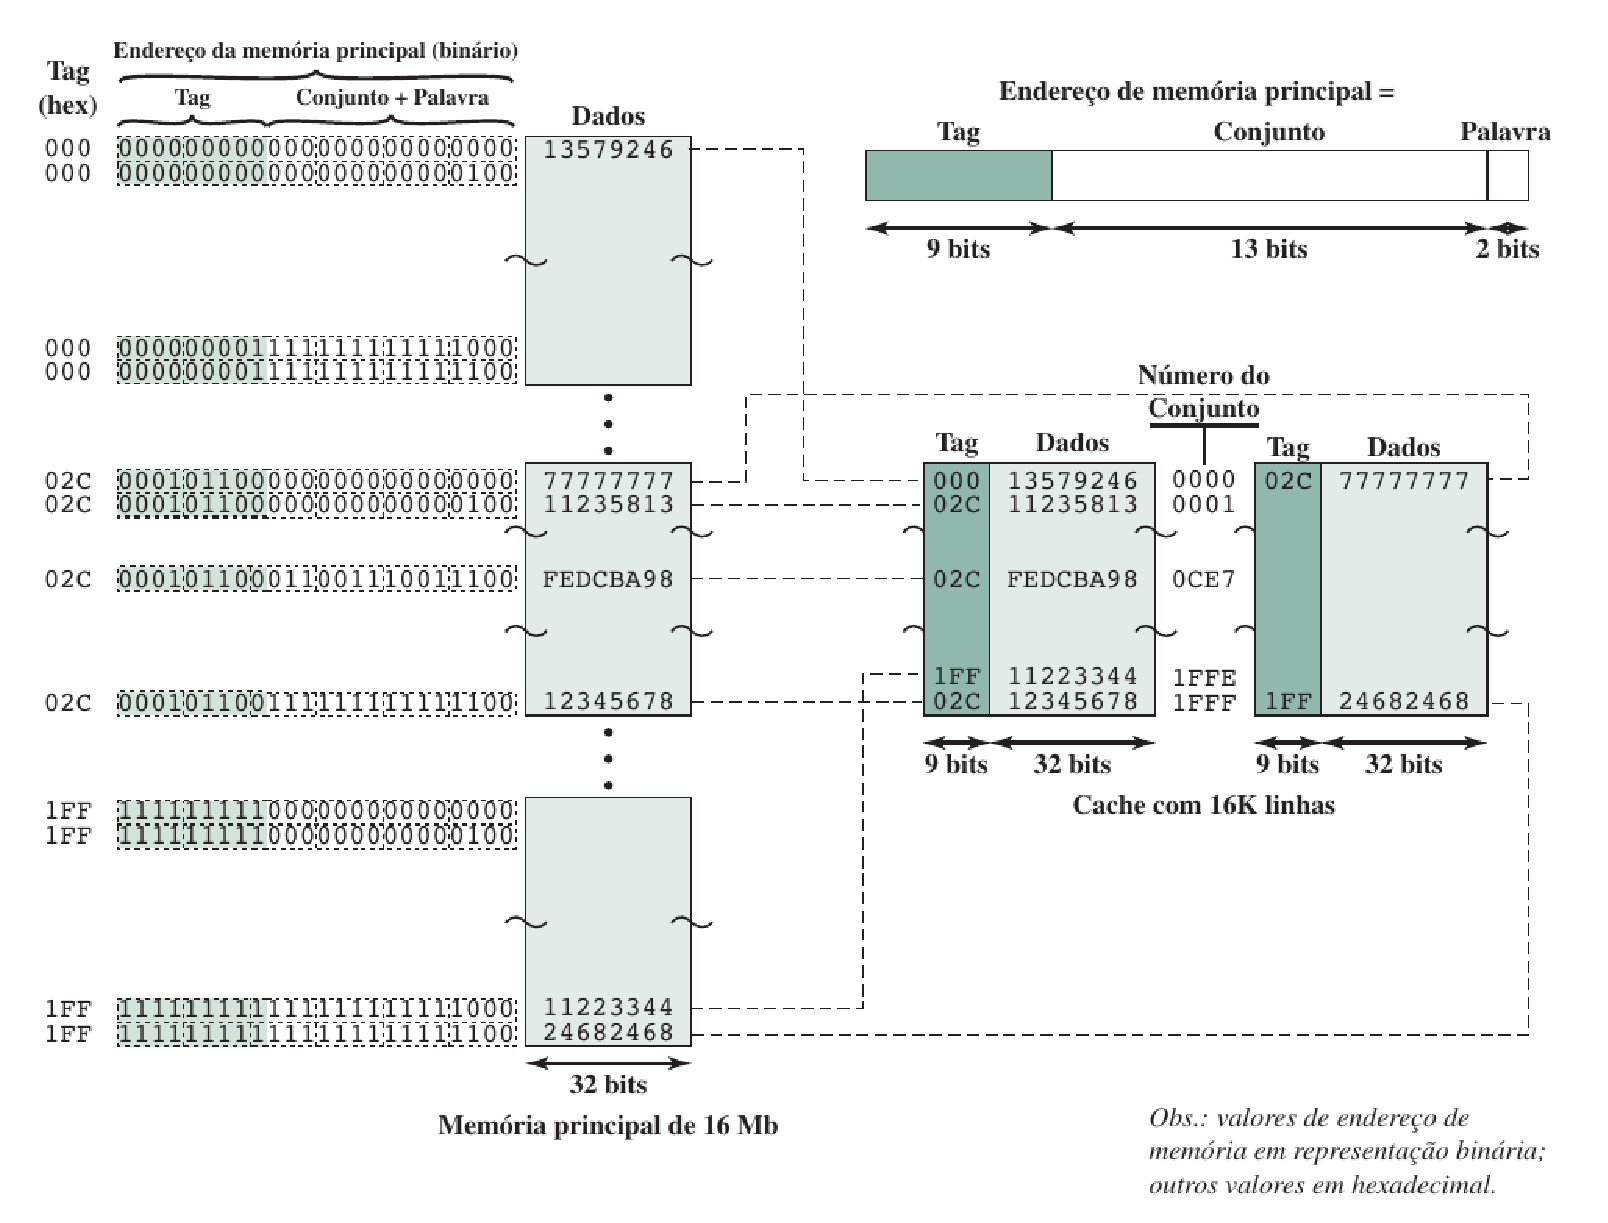
\includegraphics[height=0.5\textwidth]{figs/exemplo-associativo-conj}
	\end{center}
\end{slide}

\begin{slide}{Mapeamento associativo em conjunto}
	Organização de uma cache com mapeamento associativo em conjunto
	\begin{center}
		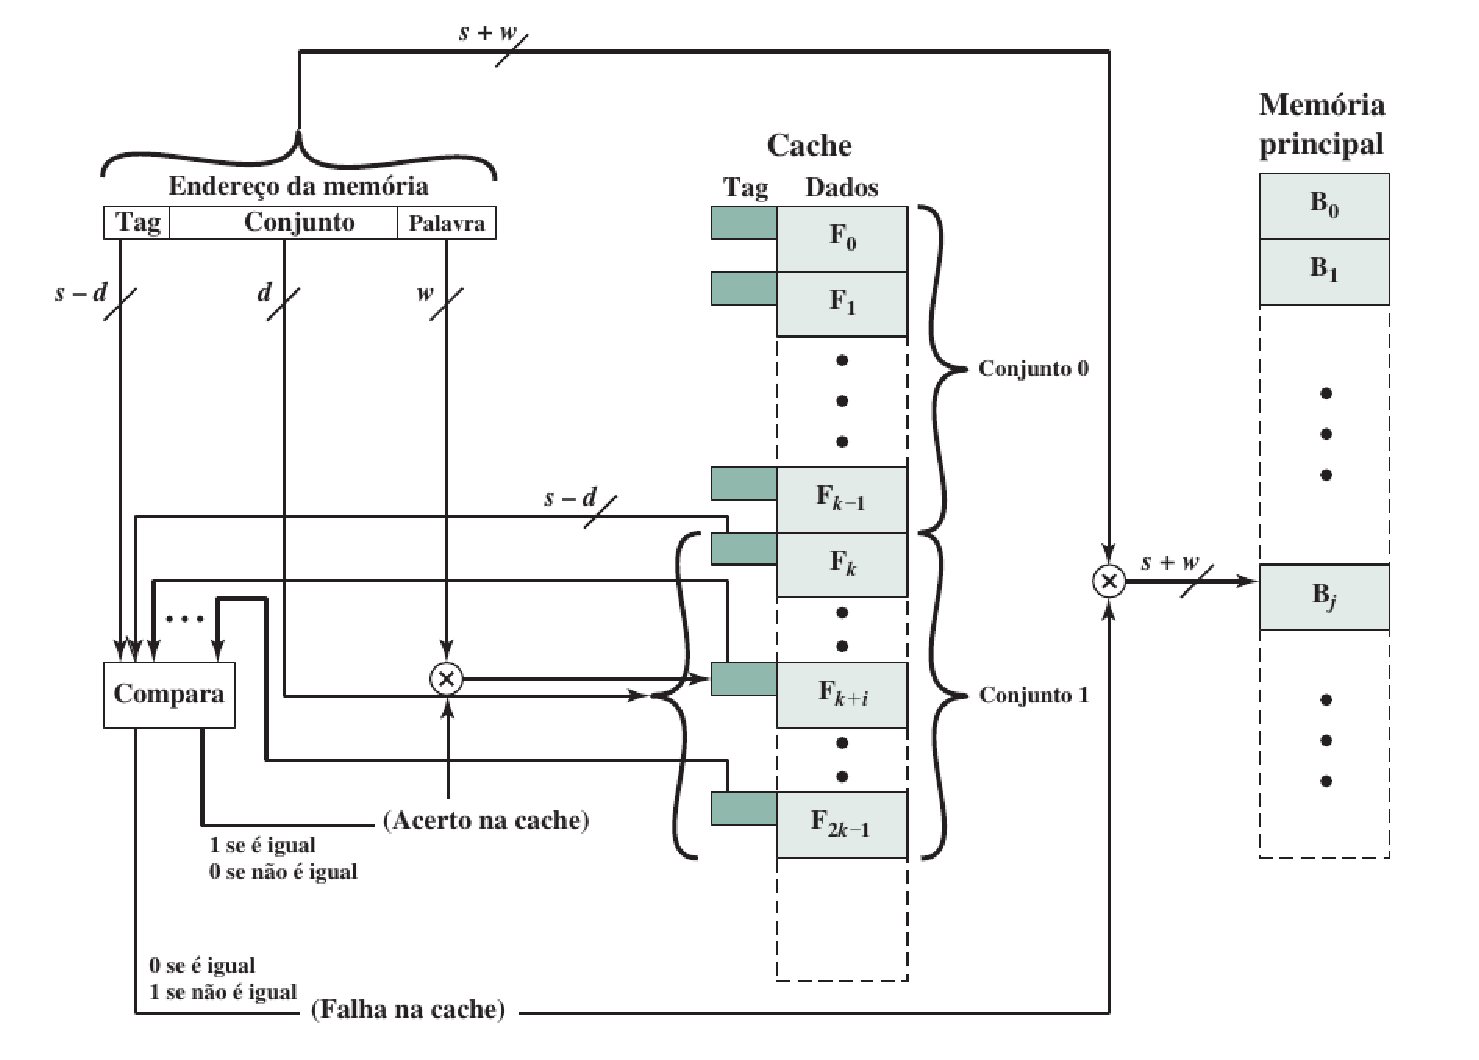
\includegraphics[height=0.5\textwidth]{figs/organizacao-associativo-conj}
	\end{center}
\end{slide}

\begin{slide}{Mapeamento associativo em conjunto}
	Comparação de \emph{hits} em relação ao tamanho da cache e o tipo de mapeamento
	\begin{center}
		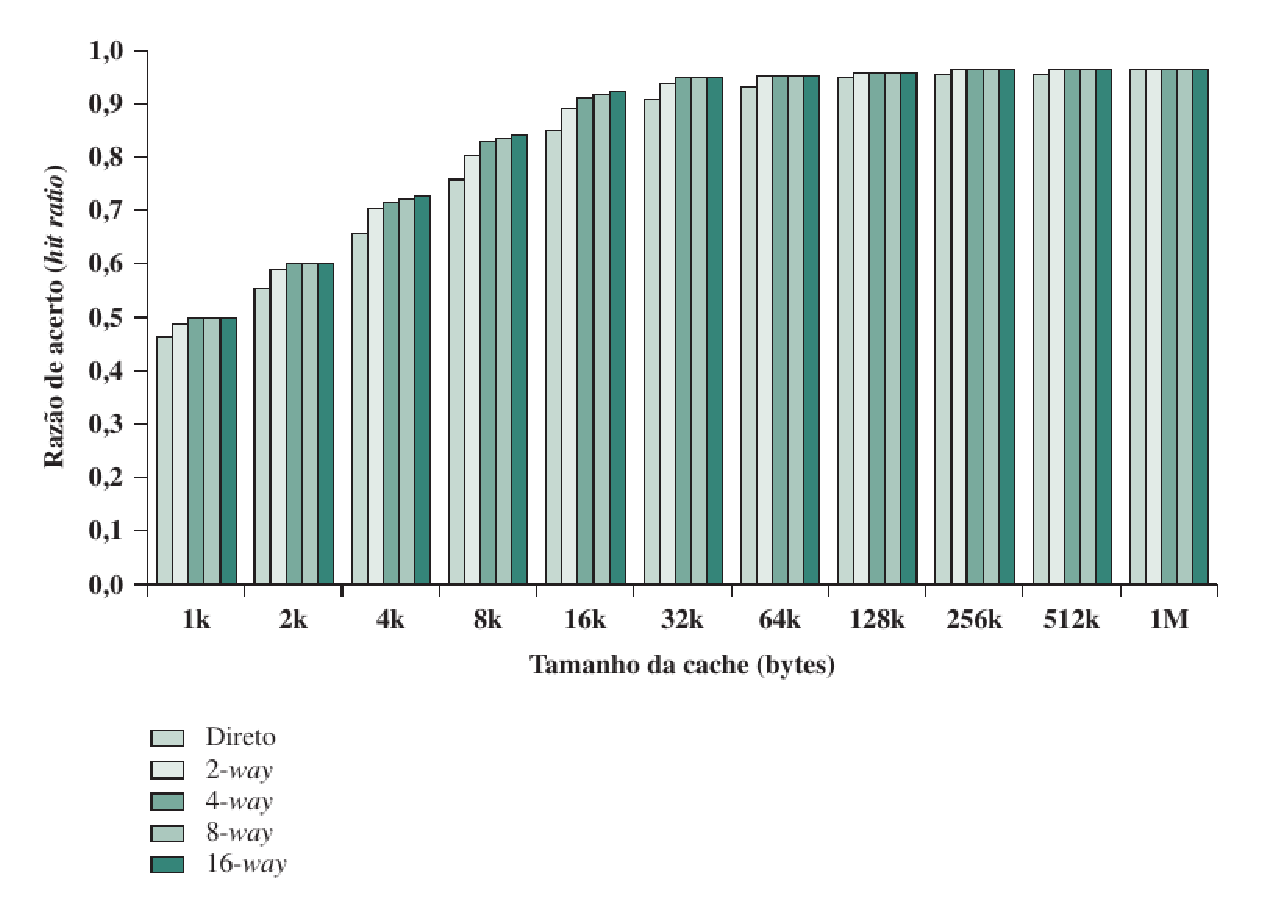
\includegraphics[height=0.5\textwidth]{figs/razao-acerto-tipo}
	\end{center}
\end{slide}

\begin{slide}{Algoritmos de substituição}
	\small
\begin{itemize}
   \item Cache cheia: quando um novo bloco é trazido para a cache, um dos blocos armazenados precisa ser substituído
   \item Se o mapeamento não for direto: um algoritmo de substituição é necessário;
   \item Implementação deve ser em \emph{hardware} para obtenção de desempenho necessário;
   \item \emph{O menos usado recentemente} (LRU): substituir o bloco no conjunto com menos referências recentes;
	   \begin{itemize}
		   \item Em conjuntos de duas linhas: emprego de \emph{use bit} para indicar a linha usada mais recentemente;
		   \item Em mapeamento associativo: lista de todos os índices de linha; a cada referência, o índice vai para o topo; a linha a substituir é a da base da lista
	   \end{itemize}
   \item \emph{Primeiro a entrar primeiro a sair}: substitua o bloco no conjunto que esteve na cache por mais tempo;
	   \begin{itemize}
		   \item Uso de uma lista circular
	   \end{itemize}
   \item \emph{O menos frequentemente usado}: substituir o bloco no conjunto que teve menos referências;
	   \begin{itemize}
		   \item Implementação de um contador para cada linha da cache
	   \end{itemize}
   \item \emph{Escolha aleatória}
\end{itemize}
\end{slide}

\begin{slide}{Política de escrita}
\begin{itemize}
   \item Substituição de um bloco da cache:
   \begin{itemize}
      \item Bloco antigo não foi alterado: pode substituir sem problema;
      \item Bloco antigo foi alterado: é necessário atualizar a memória;
   \end{itemize}
   \item Situações problema:
   \begin{itemize}
      \item Mais de um dispositivo pode ter acesso à memória (processador e E/S)
      \item Mais de um processador pode ter acesso à memória (ambiente multi processado):
      \begin{itemize}
         \item Processadores compartilham o barramento
         \item Cada um possui sua cache própria
      \end{itemize}
   \end{itemize}
\end{itemize}
\end{slide}

\begin{slide}{Política de escrita}
\begin{itemize}
   \item Write Through
   \begin{itemize}
      \item Técnica mais simples
      \item Cada operação de escrita é realizada tanto na(s) cache(s) quanto na memória principal
      \item Cada módulo processador-cache deve monitorar a atividade do barramento
      \item Desvantagem: grande tráfego de dados no barramento
   \end{itemize}
   \item Write back
   \begin{itemize}
      \item Inicialmente, a operação de escrita é feita apenas na cache
      \item Quando uma escrita é realizada em um linha da cache, o \emph{dirty bit} (ou \emph{use bit}) correspondente é \emph{setado}
      \item Quando o bloco alterado for substituído, se o \emph{dirty bit} estiver \emph{setado}, a mémória é atualizada
      \item Problema? Manutenção de coerência é difícil quando mais de um dispositivo tem acesso à memória
    \end{itemize}
\end{itemize}
\end{slide}

\begin{slide}{Política de escrita}
\begin{itemize}
   \item Abordagens possíveis para manutenção da coerência entre caches
   \begin{itemize}
      \item Monitoramento de barramento com \emph{write through}
      \begin{itemize}
         \item Cada controlador de cache monitora as linhas de endereço 
         \item Se um endereço de memória, cujo conteúdo esteja armazenado na cache, é alterado, a linha correspondente da cache é invalidada
         \item Exige que todos usem \emph{write through}
      \end{itemize}
      \item Transparência em hardware
      \begin{itemize}
         \item Hardware adicional é usado para garantir que qualquer alteração na memória via cache seja atualizada em todas as caches do sistema
      \end{itemize}
      \item Memória \emph{não cacheável}
      \begin{itemize}
         \item Somente uma parte da memória é partilhada com outros processadores
         \item A região partilhada não pode ser armazenada em cache
      \end{itemize}
   \end{itemize}
\end{itemize}
\end{slide}

\begin{slide}{Tamanho de linha}
	\begin{itemize}
		\item A razão de acerto aumenta até um limite com o aumento de tamanho da linha da cache
		\item O aumento do tamanho do bloco (linha):
			\begin{itemize}
				\item Reduz o número de blocos que cabem na cache: blocos são sobrescritos pouco depois de serem buscados
				\item As palavras que compõem um bloco estão mais distantes entre si e, portanto, menor é a probabilidades de referências futuras
			\end{itemize}
		\item A relação entre taxa de acerto e tamanho de bloco é complexa e depende das característica de localidade de cada programa sendo executado
		\item Blocos de 8 a 64 bytes são comuns. Em HPC (high performance computation), blocos de 64 a 128 bytes são frequentes
	\end{itemize}
\end{slide}

\begin{slide}{Número de caches}
	\twocolumn
	{
		\begin{itemize}
			\item Atualmente os sistemas de memória possuem mais de um nível de memória cache
			\item Tais níveis podem ser \emph{on chip} ou externos (acesso via barramento do sistema ou dedicado)
			\item Cache \emph{on chip}:
				\begin{itemize}
					\item Não sobrecarrega barramento externo
					\item Transferência de dados mais rápida para o processador (sem estados de espera)
				\end{itemize}
		\end{itemize}
	}
	{
		\begin{itemize}
			\item Validade da cache externa\\
			\begin{center}
				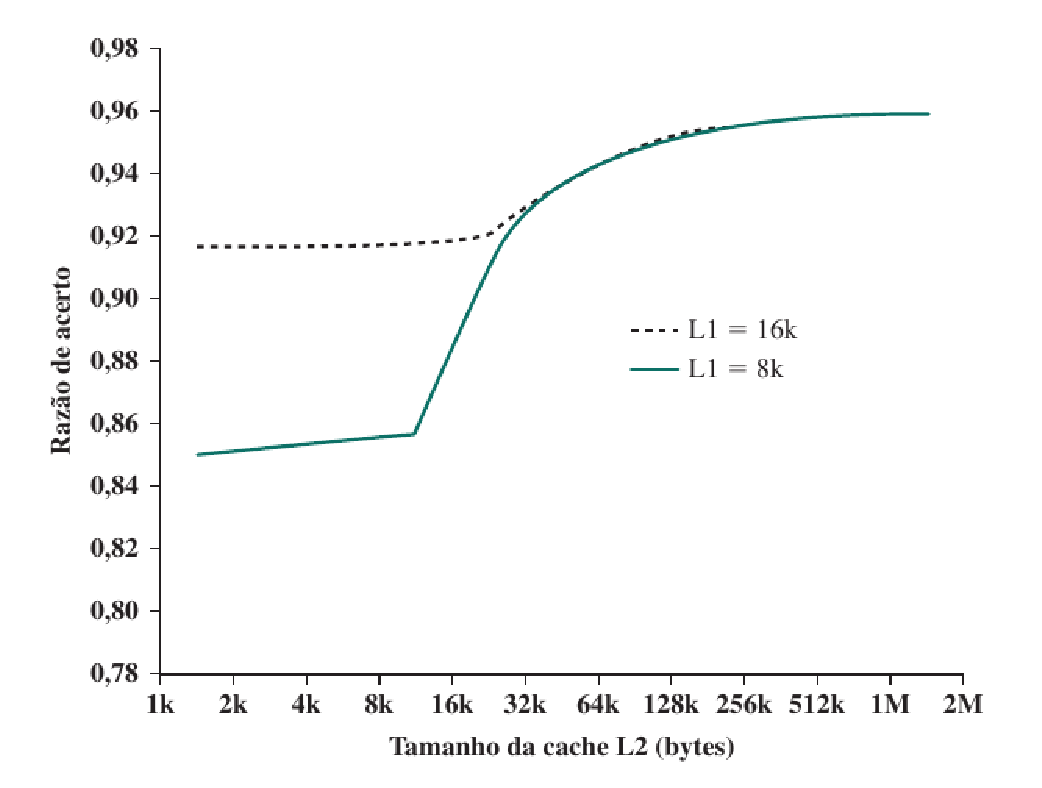
\includegraphics[width=\textwidth]{figs/acerto02}
			\end{center}
		\end{itemize}
	}
\end{slide}

\begin{slide}{Caches separadas ou unificadas}
	\begin{itemize}
		\item Cache unificada:
			\begin{itemize}
				\item Dados e intruções compartilham uma mesma cache
				\item A complexidade da interface é menor
				\item O balanço de posicões para armazenamento entre instruções e dados é feito de maneira automática
			\end{itemize}
		\item Cache separada:
			\begin{itemize}
				\item Na verdade são duas caches no mesmo nível: uma para dados e outra para instruções
				\item Interface possui complexidade maior
				\item Essencial para implementação de \emph{pipeline}, pois desacopla a unidade de busca de instruções da unidade de execução
			\end{itemize}
		\item A tendência atual:
			\begin{itemize}
				\item Cache L1 \emph{on-chip}: separada
				\item Outros níveis de cache: unificada
			\end{itemize}
	\end{itemize}
\end{slide}

\end{document}
